\chapter{Organization Overview}
\label{ch:org}

\section{History and Mission}
\label{sec:history}

Brain Station 23 (BS-23) is a prominent software development company headquartered in Dhaka, Bangladesh, with a strong focus on delivering innovative IT solutions across healthcare, e-commerce, logistics, fintech, and hospitality verticals. Founded with a vision to bridge technology and business impact, BS-23 has grown to become one of Bangladesh's leading technology exporters, serving both local enterprises and international clients across North America, Europe, and APAC.

Since inception, BS-23 has built a reputation for technical excellence, systematic problem-solving, Agile delivery discipline, and sustained customer satisfaction --- attributes directly observed during the 10-day attachment.

\begin{table}[H]
\centering
\caption{Brain Station 23 --- Organizational Profile}
\label{tab:bs23_profile}
\begin{tabularx}{\textwidth}{@{}p{0.28\textwidth}X@{}}
\toprule
\textbf{Attribute} & \textbf{Details} \\
\midrule
Company Name & Brain Station 23 (BS-23) \\
Headquarters & Dhaka, Bangladesh \\
Industry & Information Technology, Software Development, AI Integration \\
Specialization & Custom software, full-stack web/mobile, cloud-native architecture, AI/ML solutions, DevOps \\
Team Size (observed) & 300+ engineers across multiple delivery units \\
Mission & Deliver high-quality, innovative software solutions that drive measurable business growth \\
Vision & Be a leading global technology partner providing cutting-edge, ethical digital solutions \\
\bottomrule
\end{tabularx}
\end{table}

\section{Organizational Structure}
\label{sec:org_structure}

BS-23 operates a matrix organizational structure supporting efficient project delivery and cross-functional collaboration, with clear accountability between delivery, quality, and operations.

\begin{figure}[H]
\centering
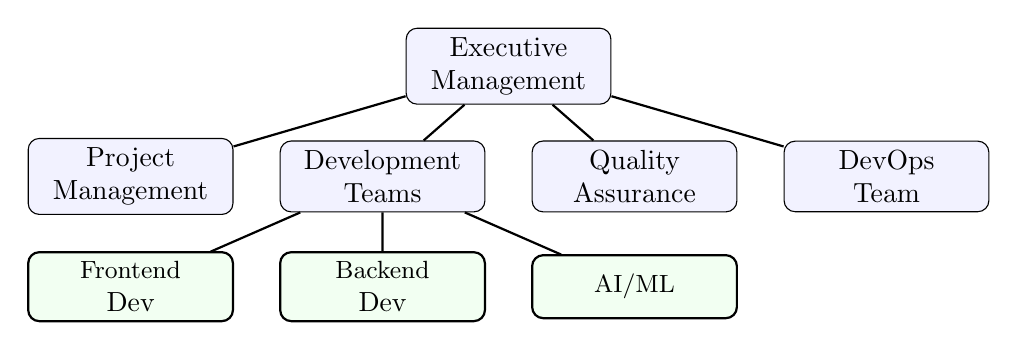
\begin{tikzpicture}[
  level distance=1.4cm,
  sibling distance=3.2cm,
  every node/.style={draw,rounded corners,align=center,minimum width=2.6cm,minimum height=0.8cm,fill=blue!5},
  edge from parent/.style={draw,thick}
]
\node {Executive\\Management}
  child { node {Project\\Management} }
  child { node {Development\\Teams}
    child { node[fill=green!5]{\small Frontend\\Dev} }
    child { node[fill=green!5]{\small Backend\\Dev} }
    child { node[fill=green!5]{\small AI/ML} }
  }
  child { node {Quality\\Assurance} }
  child { node {DevOps\\Team} };
\end{tikzpicture}
\caption{Brain Station 23 Organizational Structure}
\label{fig:org_structure}
\end{figure}

During attachment, our 7-member neoRMS squad mapped directly to this structure: a project mentor (acting PM), 3 backend engineers, 3 frontend engineers, and 1 AI engineer --- mirroring BS-23 production squads at reduced scale.

\section{Departments and Functions}
\label{sec:departments}

\subsection{Development Department}
Responsible for end-to-end software design and implementation:
\begin{itemize}
\item \textbf{Frontend Development:} React / Next.js, TailwindCSS, component design systems, accessibility (WCAG).
\item \textbf{Backend Development:} Node.js / Express, NestJS, PostgreSQL / MongoDB, Prisma / TypeORM, REST + GraphQL + WebSocket.
\item \textbf{Full-Stack Development:} cross-layer feature ownership, API contract negotiation.
\item \textbf{AI and Machine Learning Integration:} Python / FastAPI, scikit-learn, Transformers, recommendation engines, NLP pipelines --- precisely the stack used in neoRMS AI service.
\end{itemize}

\subsection{Quality Assurance Department}
Comprehensive testing: unit (Jest / Vitest), integration (Supertest), E2E, and UAT. QA engineers pair with developers throughout sprints --- shift-left quality observed in BS-23 code review culture.

\subsection{Project Management Department}
Agile Scrum formalized: sprint planning, daily stand-ups (observed 10:00 AM, 15 min time-boxed), sprint review, retrospective. JIRA / GitHub Projects used for backlog tracking. Our mentor Mohoiminul Sohol facilitated scope negotiation and blocker escalation.

\subsection{DevOps Department}
Infrastructure, CI/CD, containerization, cloud deployment (AWS / Azure), observability. Docker-first onboarding --- a practice I adopted as architect on Day 0 --- is standard at BS-23 to guarantee environment parity.

\section{Products and Services}
\label{sec:products}

\begin{table}[H]
\centering
\caption{Brain Station 23 --- Products and Services}
\label{tab:bs23_services}
\begin{tabularx}{\textwidth}{@{}p{0.30\textwidth}X@{}}
\toprule
\textbf{Service / Product} & \textbf{Description} \\
\midrule
Custom Software Development & Tailored enterprise solutions with domain-driven design \\
Web Development & Full-stack applications: React / Vue / Angular + Node / .NET / Django \\
Mobile App Development & Native and cross-platform (React Native, Flutter) \\
AI and ML Solutions & Recommendation, NLP, computer vision, predictive analytics --- as demonstrated in neoRMS \\
Cloud Solutions & AWS / Azure migration, containerization, Kubernetes, serverless \\
Consulting Services & Technology strategy, architecture review, digital transformation \\
Maintenance and Support & 24/7 SRE, observability, continuous improvement \\
\bottomrule
\end{tabularx}
\end{table}

\section{Quality and Compliance Standards}
\label{sec:compliance}

\begin{itemize}
\item \textbf{ISO 9001:2015} --- Quality management system; observed in documented code review checklists and definition-of-done criteria.
\item \textbf{Data Protection Compliance} --- GDPR principles applied: data minimization, consent management, right to erasure --- implemented in neoRMS user delete / anonymization flows.
\item \textbf{Security Standards} --- OWASP Top 10 mitigations enforced in code review: input validation (Zod), JWT with httpOnly cookies, RBAC, parameterized queries via Prisma, rate limiting discussion.
\item \textbf{Code Quality Standards} --- ESLint + Prettier enforced, conventional commits, mandatory peer review (minimum 1 approver), branch protection on \texttt{main}.
\item \textbf{Agile Compliance} --- Scrum events time-boxed, velocity tracked via GitHub Projects, retrospective action items documented.
\end{itemize}

\section{Workplace Safety and Environmental Policy}
\label{sec:safety}

\subsection{Workplace Safety Measures}
Observed during 10-day onsite/remote hybrid attachment:
\begin{itemize}
\item Ergonomic workstations: adjustable chairs, monitor arms, proper desk height.
\item 20--20--20 eye care rule actively encouraged; blue-light filters standard.
\item Clear evacuation routes, fire extinguishers, emergency contacts visibly posted.
\item Mental health: flexible hours, open mentorship, psychological safety in stand-ups --- junior suggestions evaluated on technical merit, regardless of seniority.
\item Remote work option reducing commute stress, supporting work-life balance.
\end{itemize}

\subsection{Environmental Policy}
\begin{itemize}
\item Digital-first documentation: zero paper SRS/BRD --- all Confluence / Notion / GitHub Wiki.
\item Energy-efficient hardware refresh cycle; auto sleep policies.
\item E-waste recycling program in partnership with certified vendors.
\item Remote / hybrid model promoted, measurably reducing office carbon footprint.
\item neoRMS itself contributes: digital ordering eliminates paper KOT slips; inventory optimization reduces food waste via low-stock alerts.
\end{itemize}

BS-23's operational maturity --- structured process, ethical engineering culture, and conscious sustainability --- provided an exemplary environment for transitioning from academic projects to professional system leadership.
